\chapter{Конструкторская часть}

\section{Требования к программному обеспечению}

К разрабатываемой программе предъявлен ряд требований:

\textbf{Входные данные:} Две строки

\textbf{Выходные данные:} Целое число

\begin{itemize}
	\item Заглавные и строчные символы считаются разными;
	\item Возможность обработки строк как на кириллице так и на латинице;
	\item Должна быть возможность замера процессорного времени программы;
	\item Должна быть возможность вывода графиков и таблиц замеров процессорного времени и памяти.
\end{itemize}

\section{Разработка алгоритмов}
На рисунке \ref{fig:RL} представлена схема алгоритма нахождения расстояния Левенштейна. На рисунках \ref{fig:RLC1} – \ref{fig:RLC2} представлена итерационная реализация алгоритма поиска расстояния Левенштейна. В первой части алгоритма, на рисунке \ref{fig:RLC1} представлены создание и начальное заполнение матрицы кеша.На рисунке \ref{fig:RLC2}, во второй части алгоритм, изображён цикл с заполнением матрицы и поиском расстояния. На рисунках \ref{fig:RDLC1} – \ref{fig:RDLC2} представлен алгоритм поиска расстояния Дамерау–Левенштейна. Алгоритм представлен только в итерационной вариации с использованием кеширования. Первая часть алгоритма совпадает с первой частью на рисунке \ref{fig:RLC1}. Вторая часть отличается от \ref{fig:RLC2}, тем, что в заполнение матрицы добавлена операция транспозиции соседних элементов строки.


\begin{figure}[h]
	\centering
	\includegraphics[width=0.9\textwidth]{RL}
	\caption{Схема рекурсивного алгоритма нахождения расстояния Левенштейна}
	\label{fig:RL}
\end{figure}

\begin{figure}[h]
	\centering
	\includegraphics[width=0.55\textwidth]{RLС1}
	\caption{Схема алгоритма нахождения расстояния Левенштейна с кешем, часть 1}
	\label{fig:RLC1}
\end{figure}

\begin{figure}[h]
	\centering
	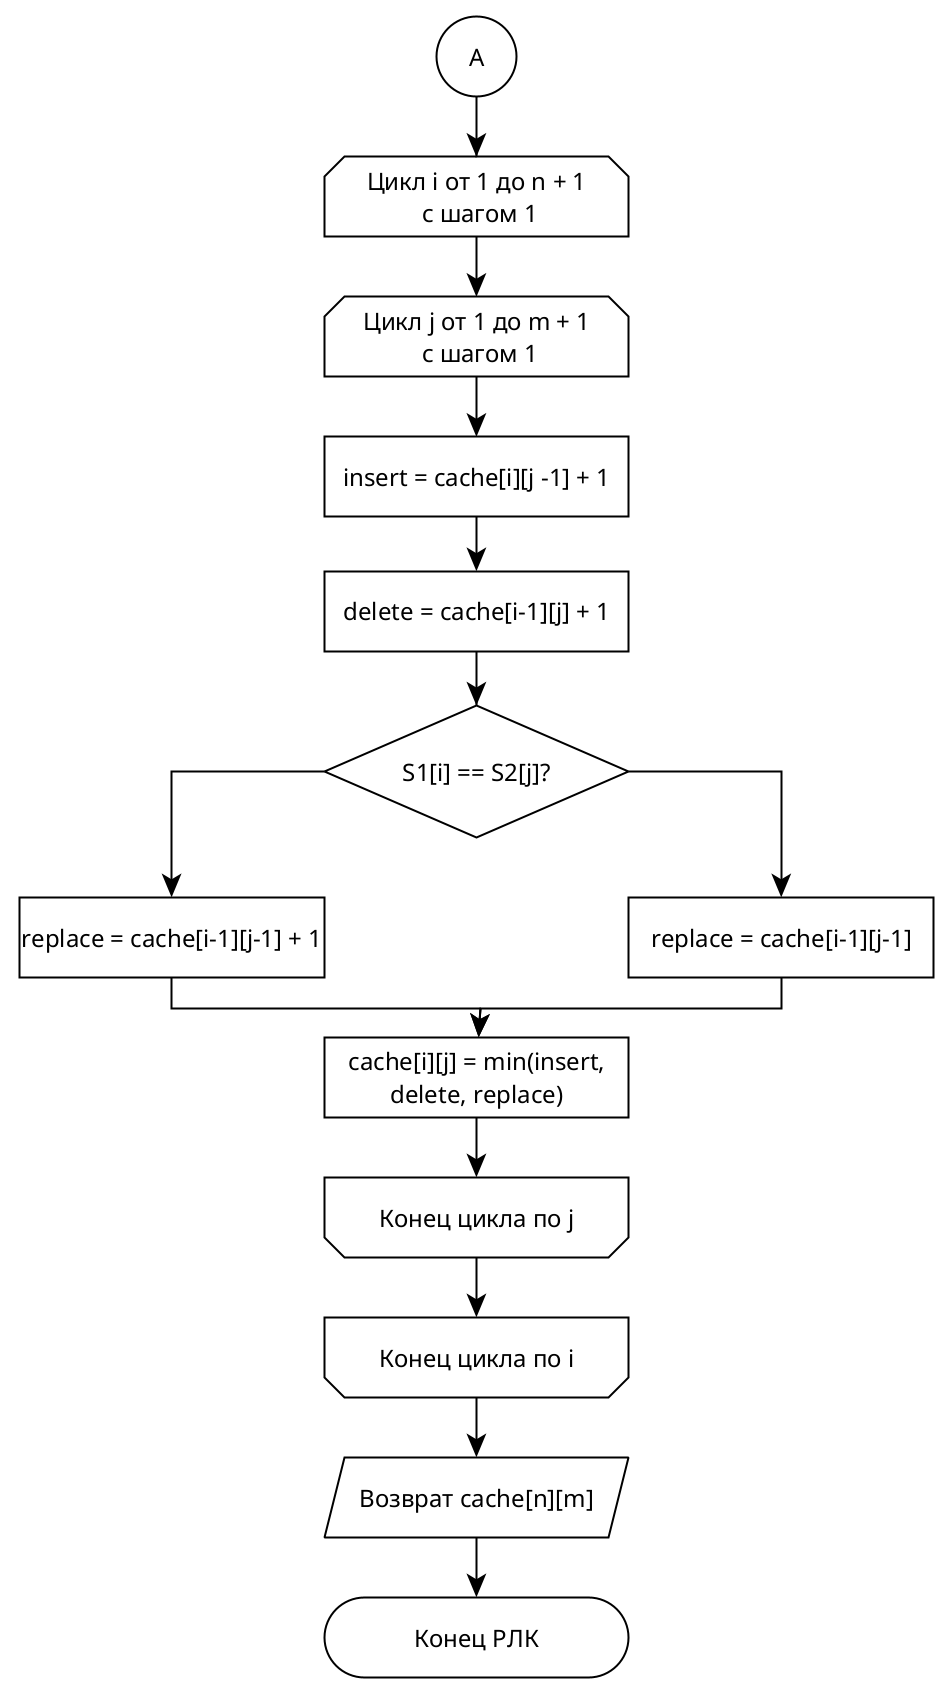
\includegraphics[width=0.7\textwidth]{RLC2}
	\caption{Схема алгоритма нахождения расстояния Левенштейна с кешем, часть 2}
	\label{fig:RLC2}
\end{figure}

\begin{figure}[h]
	\centering
	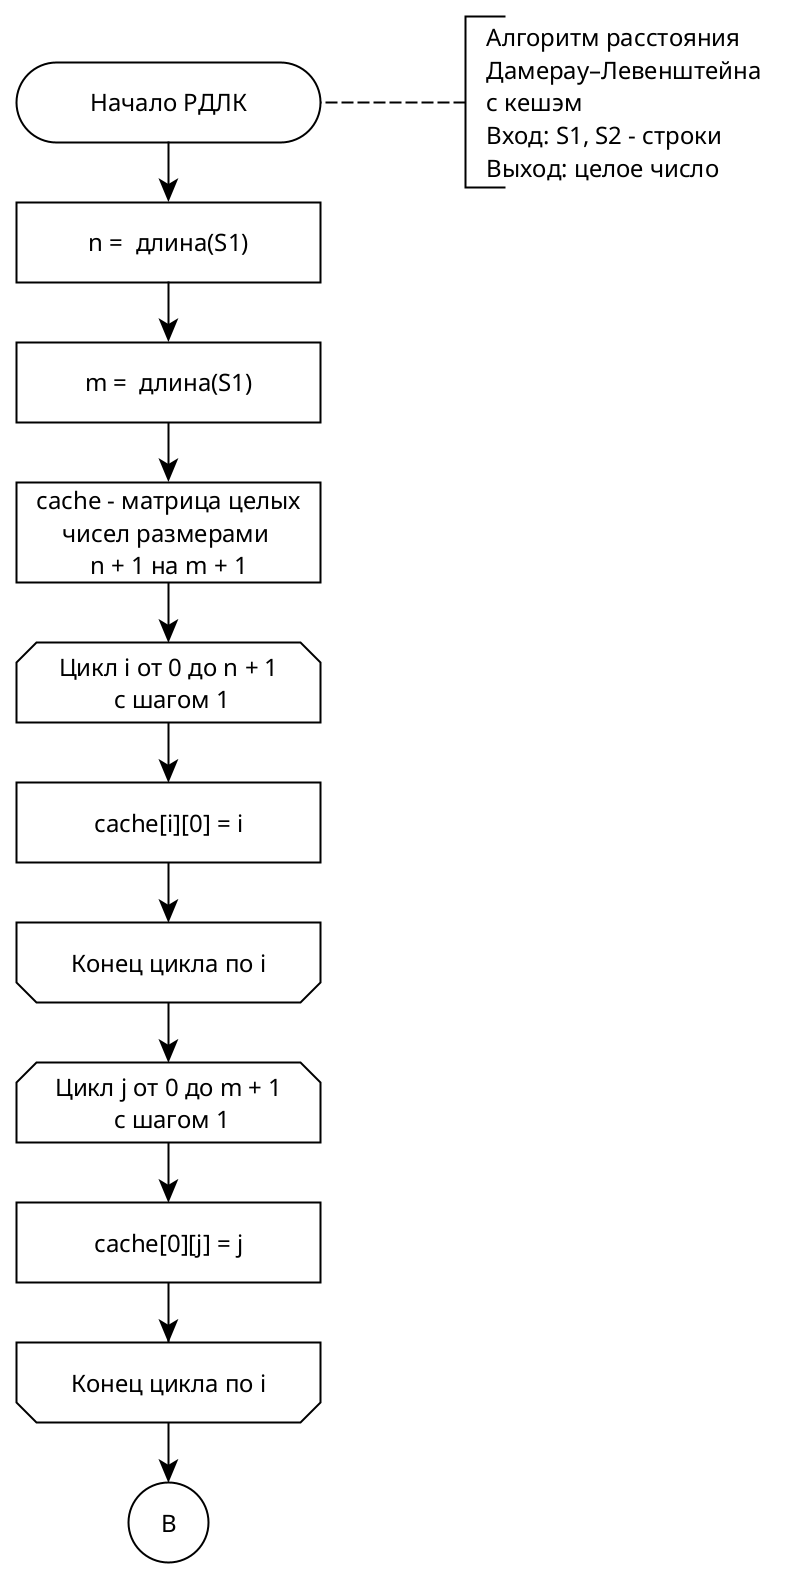
\includegraphics[width=0.55\textwidth]{RDLC1}
	\caption{Схема алгоритма нахождения расстояния Дамерау–Левенштейна с кешем, часть 1}
	\label{fig:RDLC1}
\end{figure}


\begin{figure}[t]
	\centering
	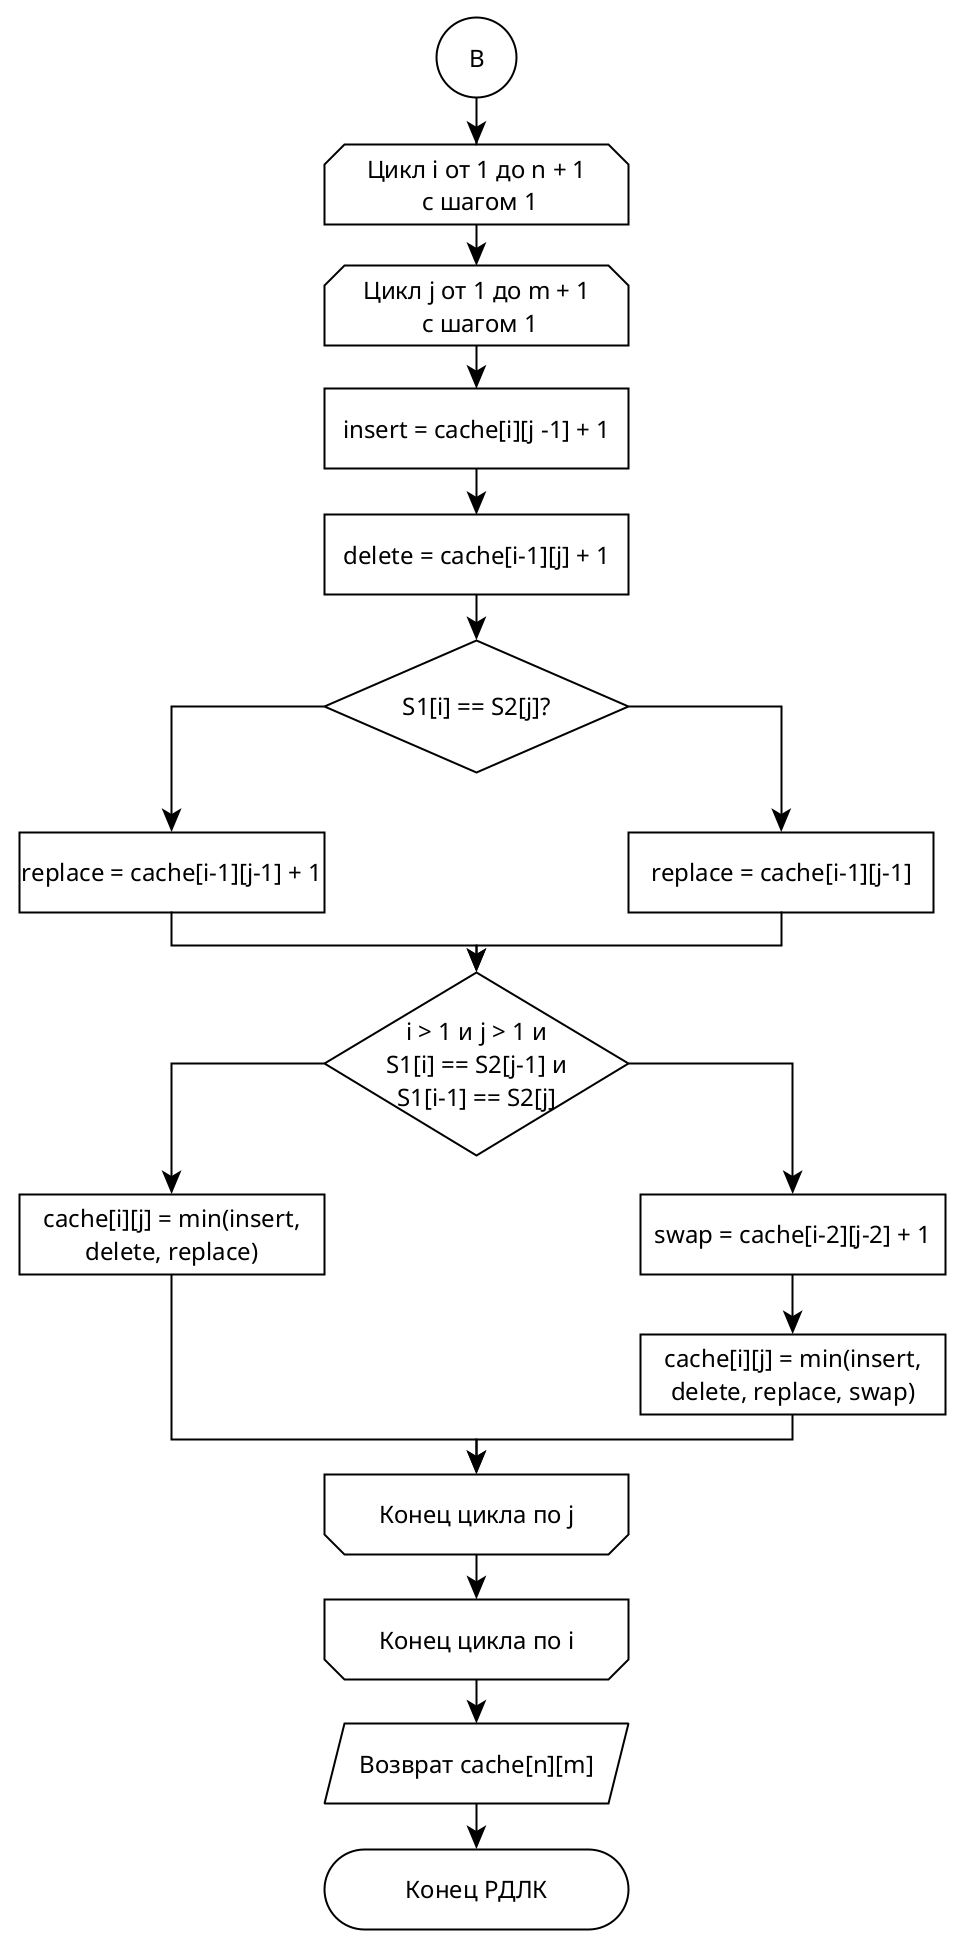
\includegraphics[width=0.7\textwidth]{RDLC2}
	\caption{Схема алгоритма нахождения расстояния Дамерау–Левенштейна с кешем, часть 2}
	\label{fig:RDLC2}
\end{figure}

\clearpage


\section{Вывод}

В результате конструкторской части были определены требования к ПО, а также разработаны схемы алгоритмов рекурсивного поиска расстояния Левенштейна, итерационного поиска с кешем и итерационного алгоритма поиска расстояния Дамерау–Левенштейна с кешем.

\clearpage
